\chapter{Towards verifyng Bitcoin-S with Stainless}
\label{chap:connecting}

\section{Integration (Versionskonflikte, neues Plugin)}


\section{Error Reporting with sbt and JAR}


\section{Trying to Verify checkTransaction}

\subsection{Findings}


\subsection{Bugfix}


\section{Verification of Method "+ 0" // Change this}
After so many failures, we have decided to search for the smallest unit in Bitcoin-S-Core that is worthwhile to verify.
We found the addition of two Satoshis would be a good candidate.
To make it even more easy, we decided to verify only the addition, where we add zero to an amount of Satoshis.
The signature looks like the following.
\begin{lstlisting}
  +(c: CurrencyUnit): CurrencyUnit
\end{lstlisting}
Where the class Satoshis extends CurrencyUnit.
The post condition would be, that the parameter c must be zero.
\begin{lstlisting}
  require(c.satoshis.underlying == Int64.zero)
\end{lstlisting}
\emph{c.satoshis} is an abstract method of CurrencyUnit that must return an instance of the class Satoshis.

\emph{c.satoshis.underlying} is also an abstract method of CurrencyUnit that must return an instance of the abstract type A.

Both are implemented in Satoshis where A is set to Int64.
So the underlying number of the parameter must be zero.

Next we ensure, that the result is the same value as \emph{this}.
\begin{lstlisting}
  ensuring(res => res.satoshis == this.satoshis)
\end{lstlisting}
Here, we can directly use equals (==) on Satoshis, because its a case class and Int64, the only parameter of Satoshis is a case class too.

After writing the verification, we ran Stainless on the source files.
It prints a lot of errors because of code incompatibility.
So we had to rewrite it as described in the following sections.

\subsection{Rewriting Abstract Type Member}
Stainless output:
\begin{lstlisting}
[ Error  ] CurrencyUnits.scala:5:3: Stainless doesn't support abstract type members
           type A
\end{lstlisting}
This should be easy to rewrite by using generics instead of an abstract type, right?
Unfortunately not.
The problem is, CurrencyUnit uses its implementing class Satoshis.

Simplified code.
\begin{lstlisting}
  sealed abstract class CurrencyUnit {
    def +(c: CurrencyUnit): CurrencyUnit =
      Satoshis(satoshis.underlying + c.satoshis.underlying)
  }

  sealed abstract class Satoshis extends CurrencyUnit
\end{lstlisting}
Thus, when we use generics, Satoshis is not of type CurrencyUnit anymore and neither of type CurrencyUnit[A], where A is the new generic type.
Satoshis extends CurrencyUnit with type Int64, so it is of type CurrencyUnit[Int64].
That's to specific.

Since there is no easy way to fix it and the code should stay as much as possible the original, we decided to remove the abstract type.
The verification is a bit more limited, to only Satoshis, but that's no problem, because the goal is to verify the addition of Satoshis.

So by removing the abstract type and fix it to Int64 as defined by Satoshis, there was one error less in Stainless.

\subsection{Rewriting Generics}
// I dont understand this.. maybe just a missing feature in Stainless?
Stainless output:
\begin{lstlisting}
  [ Error  ] NumberType.scala:3:30: Unknown type parameter type T
             sealed abstract class Number[T <: Number[T]]

\end{lstlisting}

\begin{lstlisting}
  sealed abstract class Number[T <: Number[T]] extends BasicArithmetic[T]  
\end{lstlisting}

\subsection{Rewriting Objects}
// TODO reason? because we can not extend case object?

Stainless output:
\begin{lstlisting}
[ Error  ] CurrencyUnits.scala:54:1: Objects cannot extend classes or implement
           traits, use a case object instead
           object Satoshis extends BaseNumbers[Satoshis] {
\end{lstlisting}

\subsection{Rewriting BigInt Constructor (only literal argument, no long argument, etc.)}
Stainless output:
\begin{lstlisting}
[ Error  ] CurrencyUnits.scala:47:33: Only literal arguments are allowed for BigInt.
           def toBigInt: BigInt = BigInt(toLong)
\end{lstlisting}
As described before, Stainless supports only a subset of Scala.
They provide their own dedicated BigInt library.
This library does not have support for dynamic BigInt construction only for string literals.

Again, a simplified version.
\begin{lstlisting}
  sealed abstract class Satoshis extends CurrencyUnit {
    def toBigInt: BigInt = BigInt(toLong)
    def toLong: Long = underlying.toLong
  }

  object Int64 extends BaseNumbers[Int64] {
    private case class Int64Impl(underlying: BigInt) extends Int64
  }
\end{lstlisting}
This would be really hard to refactor, because Bitcoin-S-Core tries to be as much dynamic as possible so it can be used with other cryptocurrencies too.
Maybe it would even be impossible, because they need to parse a lot from the bitcoin network.

Restricting the code one more time helps.
\emph{toBigInt} can directly return underlying, because in case of Int64, which is what Satoshis use, it is a BigInt.
So it does not be converted from BigInt to Long and back to BigInt.

\subsection{Rewriting Private Inner Classes}
Stainless output (simplified):
\begin{lstlisting}
  [Warning ] CurrencyUnits.scala:36:3: Could not extract tree in class:
             case private class SatoshisImpl extends Satoshis
\end{lstlisting}
Stainless is not able to extract private classes inside other objects.
Bitcoin-S-core uses it a lot, because they separate the class from its implementation.
\begin{lstlisting}
  object Int64 extends BaseNumbers[Int64] {
    private case class Int64Impl(underlying: BigInt) extends Int64 
  }
\end{lstlisting}
This is an easy one.
Just extract the inner class out of the object.
This is not exactly the same code but since the class is still private it can not be extended outside of the file.

\subsection{Rewriting Type Member}
Stainless output:
\begin{lstlisting}
  [Warning ] NumberType.scala:5:3: Could not extract tree in class: type A
             = BigInt (class scala.reflect.internal.Trees$TypeDef)
             type A = BigInt
\end{lstlisting}
Since the type A is not overridden in any of its subclasses, this can simply be hard coded.
\begin{lstlisting}
  sealed abstract class Number {
    type A = BigInt
    protected def underlying: A
    def apply: A => T
  }
\end{lstlisting}
Replace every occurence of A with BigInt.
This might be a missing feature in Stainless that should not be to hard to fix.
There is an open pull request \mypound470 on Github for this issue.

\subsection{Rewriting Usage of BigInt \&-Function}
Stainless output:
\begin{lstlisting}
  [ Error  ] NumberType.scala:19:14: Unknown call to & on result (BigInt) with
             arguments List(Number.this.andMask) of type List(BigInt)
             require((result & andMask) == result,
\end{lstlisting}
Due to the restrictions on BigInt, the \& function on it is not supported too.
\begin{lstlisting}
  sealed abstract class Number extends BasicArithmetic[Int64] {
    def andMask: BigInt

    override def +(num: Int64): Int64 = apply(checkResult(underlying + num.underlying))

    private def checkResult(result: BigInt): BigInt = {
      require((result & andMask) == result, "Result was out of bounds, got: " + result)
      result
    }
  }
\end{lstlisting}
This is a bound check.
It checks, if the result of the addition is in range of the specified type (Int64 here).
So here the \& mask can be replaced with a bound check whether the result is in range of Long.MinValue and Long.MaxValue.
Again the code gets a bit more static but for this usecase its ok.

\subsection{Rewriting require}
Stainless output:
\begin{lstlisting}
  [Warning ] NumberType.scala:54:3: Could not extract tree in class:
             scala.this.Predef.require(Int64Impl.this.underlying.<=(
             math.this.BigInt.long2bigInt(9223372036854775807L)),
             "Number was too big for a int64, got: ".+(Int64Impl.this.underlying))
             (class scala.reflect.internal.Trees$Apply)
             require(underlying <= 9223372036854775807L,
\end{lstlisting}
This is, because Stainless does not support require with a second String parameter.
Removing this String fixes the error.

\subsection{Propagate require}
Finally the code works with Stainless.
But there is another problem.
Bitcoin-S-Core uses require like a fail-fast method where as Stainless needs it to verify the code.

Stainless output:
\begin{lstlisting}
  [Warning ] Found counter-example:
  [Warning ]   thiss: { x: Object | @unchecked isNumber(x) } -> Int64Impl(0)
  [Warning ]   num: { x: Object | @unchecked isInt64(x) }    -> 
                 Int64Impl(9223372036854775808)
\end{lstlisting}
Corresponding code:
\begin{lstlisting}
  sealed abstract class Number extends BasicArithmetic[Int64] {
    override def +(num: Int64): Int64 = apply(checkResult(underlying + num.underlying))

    private def checkResult(result: BigInt): BigInt = {
      require(
        result <= BigInt("9223372036854775807")
        && result >= BigInt("-9223372036854775808")
      )
      result
    }
  }
\end{lstlisting}
But how can Stainless find a counter example ignoring the require in checkResult?
Since Stainless is a static verification tool, it tests every possibility.
So it can use a number bigger than the maximum Int64 and pass it to the addition.
The require in checkResult will then fail.
Thus, the addition need to have the restrictions of checkResult too.
\begin{lstlisting}
  override def +(num: Int64): Int64 = {
    require(
      num.underlying <= BigInt("9223372036854775807")
      && num.underlying >= BigInt("-9223372036854775808")
      && this.underlying <= BigInt("9223372036854775807")
      && this.underlying >= BigInt("-9223372036854775808")
    )
    apply(checkResult(underlying + num.underlying))
  }
\end{lstlisting}
Stainless finds another counter example:
\begin{lstlisting}
  [Warning ] Found counter-example:
  [Warning ]   num: { x: Object | @unchecked isInt64(x) }    -> Int64Impl(1)
  [Warning ]   thiss: { x: Object | @unchecked isNumber(x) } ->
                 Int64Impl(9223372036854775807)
\end{lstlisting}
Sure, it can just add one to the maximum Int64 and the require does not hold anymore.
The goal is to check the addition of zero so lets add a restriction for num to be zero.

Finally, it works and verifies correctly.

\section{Result}
\begin{figure}[H]
	\centering
		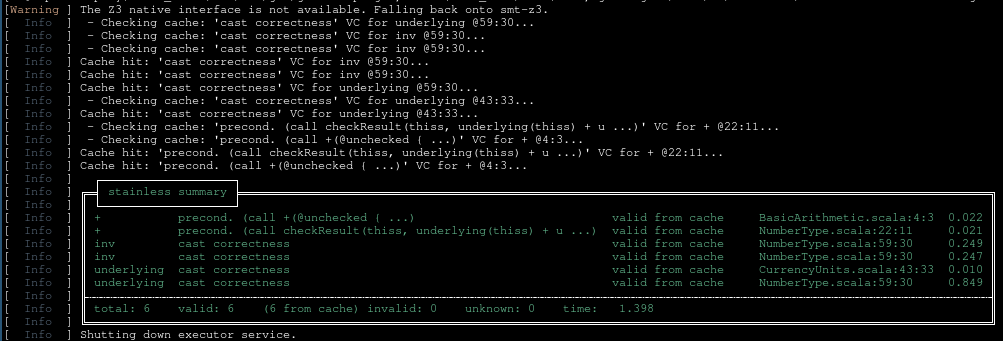
\includegraphics[scale=0.45]{images/final_verify_output.png}
	\caption{Output of Stainless verification for addition with 0 of Bitcoin-S-Cores CurrencyUnit}
	\label{fig:output1}
\end{figure}
